\subsection{Coherence} \label{supervised_approach_coherence}

In this section, we implement the coherent model \cite{giunchiglia2020coherent}, which was explained in section \ref{hmc_forward}. Its contributions consist of a further layer after the model output, where the hierarchy is enforced upon the results, and a modification of the \acrfull{bce} loss function. Our initial model can thus be left intact, as we are only adding one last layer on top of it. This last layer, called \acrfull{mcm}, changes the assignment probability of each subject to be the maximum of its own probability and that of its descendants in the subject hierarchy. The formula can be found in section \ref{hmc_forward}.

We first discuss the implementation of the coherent model, and then run two experiments, where we combine the loss function of the coherent model, the \acrfull{mcl}, with the \acrfull{asl}.

\subsubsection{Implementation}

In practice, the \acrshort{mcm} is implemented as a matrix, where each row has ones for the subject it represents and its descendants, and zeros otherwise. Each row of this matrix is multiplied element-wise with the output of the model. Then, the maximum of each row is assigned to the corresponding subject. The \acrfull{mcl} modifies \acrshort{bce} loss to also ensure that the assignment probabilities respect the subject hierarchy, just as the \acrshort{mcm}. Thus, we can also extend it with the asymmetry between positive and negative samples, i.e. we can combine it with the \acrfull{asl}.

We therefore run two experiments. We first train this model with the \acrshort{mcl} as presented in the paper \cite{giunchiglia2020coherent}, and then run it again, with the \acrshort{mcl} combined with the ASL, i.e. the \acrfull{aml}. This means that the \acrshort{bce} is extended with the hierarchy constraints and also with the $\gamma$ parameters with which we weighted positive and negative samples in the previous section, as shown in the formula above.

\subsubsection{Experiments}

\begin{figure}
  \begin{subfigure}[t]{.5\textwidth}
    \centering
    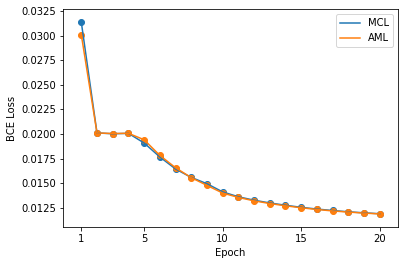
\includegraphics[width=\textwidth]{figures/supervised_approach/mcl_train_loss.png}
    \caption{Training loss}
    \label{fig:mcl_train_loss}
  \end{subfigure}
   \begin{subfigure}[t]{.5\textwidth}
    \centering
    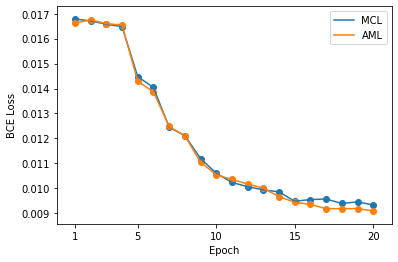
\includegraphics[width=\textwidth]{figures/supervised_approach/mcl_test_loss.png}
    \caption{Testing loss}
    \label{fig:mcl_test_loss}
  \end{subfigure}
  \caption{Test and training loss of coherent models with different gamma values.}
  \label{fig:mcl_train}
\end{figure}

\begin{figure}
  \begin{subfigure}[t]{.32\textwidth}
    \centering
    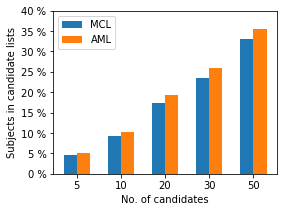
\includegraphics[width=\textwidth]{figures/supervised_approach/mcl_hw.png}
    \caption{Handwritten subjects}
    \label{fig:mcl_hw}
  \end{subfigure}
  \begin{subfigure}[t]{.32\textwidth}
    \centering
    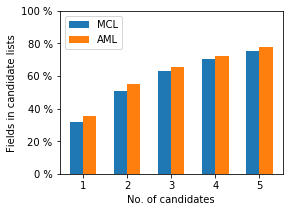
\includegraphics[width=\textwidth]{figures/supervised_approach/mcl_ddc.png}
    \caption{DDC subjects}
    \label{fig:mcl_ddc}
  \end{subfigure}
   \begin{subfigure}[t]{.32\textwidth}
    \centering
    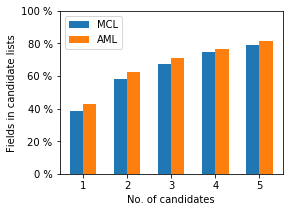
\includegraphics[width=\textwidth]{figures/supervised_approach/mcl_venue.png}
    \caption{Venues}
    \label{fig:mcl_venue}
  \end{subfigure}
  \caption{Hit rate of coherent models in the evaluation sets for different gamma values.}
  \label{fig:mcl_eval}
\end{figure}

The model used for these experiments is the same one as in section \ref{supervised_approach_asymmetric}, where we tested the asymmetric loss. The only difference is the addition of the \acrshort{mcm} layer on top of the model, and the different loss function. We have trained two models: one with the loss function from the paper \cite{giunchiglia2020coherent}, the \acrshort{mcl}, and one where the \acrshort{mcl} is combined with the \acrshort{asl}, which we call \acrfull{aml}. The parameters for the \acrshort{aml} are the ones that yielded the best results in our experiments with the \acrshort{asl}: $\gamma_+=1$ and $\gamma_-=2$.

As shown in figure \ref{fig:mcl_train}, the training procedures of both models are very similar. Both models start and end with similar training and testing losses, and also behave similarly throughout the 20 epochs both models were trained. However, the hit rate of the models on the evaluation sets favor the model trained with the \acrshort{aml}, which outscores its symmetric version for all evaluation sets and all number of candidates. The difference on the field evaluation sets is of 4 \% when only one candidate is considered, and of 2 \% on the handwritten evaluation set, when 50 candidates are considered. We therefore conclude that combining the \acrshort{asl} and \acrshort{mcl} yields the most accurate coherent model.